
This section uses the measurement setups described in Section~\ref{sec:setup} to illustrate the usefulness and repeatability of the SAVAT metric. It describes general SAVAT properties and demonstrates SAVAT's consistency across repeated measurements on one system as well as between two different systems with the same design. Section~\ref{sec:dutycycle} shows the effect of changing the duty cycle of the benchmark (the time instruction A is active vs the time instruction B is active), and shows that SAVAT does not change significantly if we exchange the order of instructions A and B in the microbenchmarks. Section~\ref{sec:freq} explains the impact of the alternation frequency on SAVAT. %Finally, Section~\ref{sec:distance} shows that SAVAT sources in computer systems can be modelled as a combination of Hertzian and magnetic dipoles and measures SAVAT as a function of measurement distance.

Practical usage of SAVAT requires that measurements taken on a single system are repeatable and consistent (precise). The tables in section~\ref{savat-20cm} showed the SAVAT values for 4 laptops and desktops. To generate these tables, SAVAT was measured 10 times for each instruction pair at a $80~{\rm kHz}$ alternation frequency and at a distance of $10~{\rm cm}$, measured on the four tested computer systems in Table~\ref{pc_specs}. The tables in Section~\ref{savat-20cm} show the means of each set of measurements for a given A/B instruction pair. Figure~\ref{fig:Variation} plots these means, along with the standard deviation among the 10 repeated measurements of each A/B instruction pair. Each point indicates the mean and standard deviation of one population of 10 SAVAT measurements (i.e. one entry in Table~\ref{fig:savat-20cm-lx61}). The position along the $x$-axis represents the mean and the $y$-axis position indicates the standard deviation for each SAVAT value. The precision is good (stdev/mean $<$ 10\%), so the resulting SAVAT values can be used to guide design decisions with confidence. This also implies that our measurements are repeatable, and indicates that the signal created by the alternation loop (discussed in the previous paragraph) is the dominant source of error in the measured SAVAT values.

\begin{figure}[htb]
  \centering
  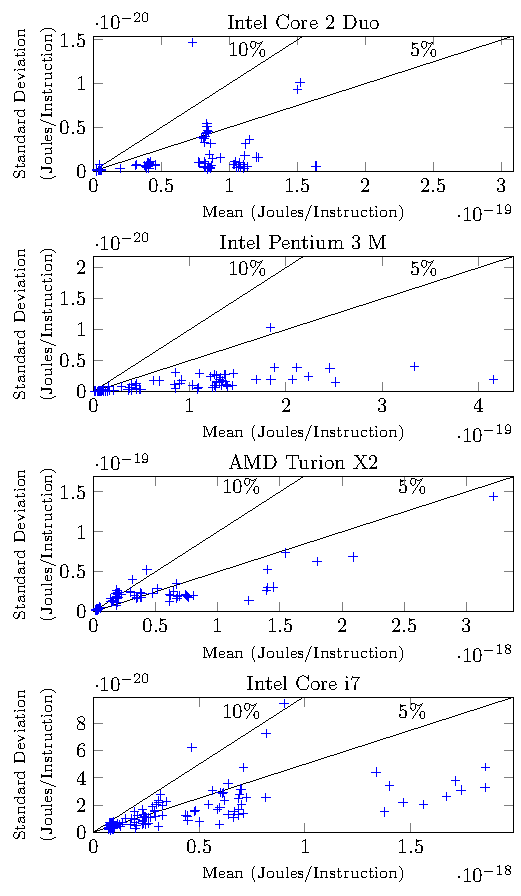
\includegraphics[width=3in]{../TEMC_SAVAT/figures/variation.pdf}
  \caption{SAVAT measurement precision.}
  \label{fig:Variation}
\end{figure}

SAVAT values must also be consistent between different physical units of the same system design for SAVAT to be practical. Figure~\ref{fig:2PCs} compares SAVAT values from two PCs (2 physical units of a DELL Optiplex 7010 model with Core i7 processors) for three different alternation frequencies using the 20 cm loop antenna. For each alternation frequency and PC, the SAVAT values have been separately normalized by the equation $\textrm{SAVAT}_{plot} = \textrm{SAVAT}_{measured}/\mu_{A/B}$ %, where $\mu_{A/A}$ is the mean of all A/A measurements (diagonal entries in Figure~\ref{fig:C2D-10-80-Table})
where $\mu_{A/B}$ is the mean of all A/B measurements where A and B are different (i.e. the off-diagonal entries in Table~\ref{fig:savat-20cm-d7010}). The black line corresponds to a perfect 1-to-1 match, and the closeness of the data points to this line indicates there is a good match between the two systems for all three alternation frequencies. This implies that SAVAT values measured on one physical system can represent all manufactured systems of the same or similar design and that our measured SAVAT values are largely insensitive to the alternation frequency.

\begin{figure}[htb]
  \centering%
  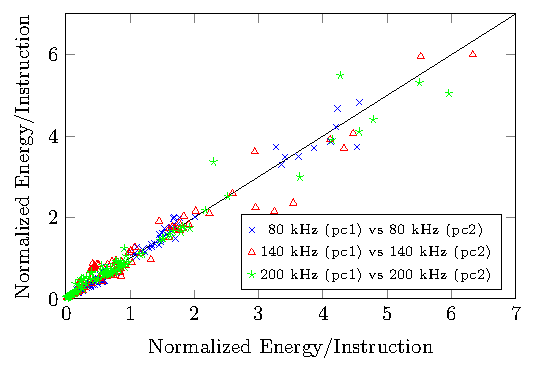
\includegraphics[width=5in]{../TEMC_SAVAT/figures/two_pcs.pdf}
  \caption{SAVAT comparison for two identical desktop (DELL Optiplex 7010) systems.}%
  \label{fig:2PCs}
\end{figure}

\subsubsection{Impact of A/B Duty Cycle and Instruction Ordering}\label{sec:dutycycle}

When measuring SAVAT the A and B instructions are each executed the same number of times per each loop iteration (\texttt{n\_inst}) because this allows us to directly calculate the energy per each executed instruction using the derivation in Appendix~\ref{appendix}. However, it is also possible to execute more A instructions than B instructions or vice versa. This changes the duty cycle for the $w[n]$ waveform described in Appendix~\ref{appendix}. Changing this duty cycle changes the magnitude of $W[1]$ and therefore changes the magnitude of $V[1]$ and the measured spectral power. 

\begin{figure}[htb]
\centering
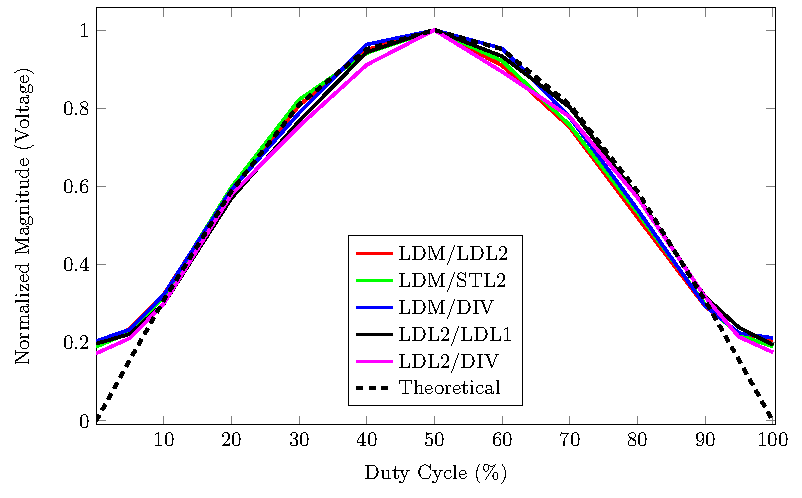
\includegraphics[width=5in]{../TEMC_SAVAT/duty_fit.pdf}
\caption{The effect of the alternation waveform duty cycle on observed SAVAT.}
\label{duty_fit}
\end{figure}

The effect of the duty cycle on different pairs of instructions is illustrated in Figure~\ref{duty_fit}. These results were obtained by varying the duty cycle of several A/B pairs and observing the change in power as a function of duty cycle. The duty cycle was varied by executing the A and B instructions different numbers of times per each iteration of the alternation loop. For example, if executing LDL1 and LDL2 $100$ times each per loop iteration results in a duty cycle of $50\%$, then executing LDL1 50 times and LDL2 150 times per iteration results in a duty cycle of $25\%$. Each instruction pair has a different maximum magnitude (as seen in the SAVAT tables) and so the general trend is best seen by normalizing each curve so that the power observed at $50\%$ duty cycle is plotted at 1.

These experimental values can be compared against the theoretical curve using Fourier analysis of square waves with varying duty cycle. From Fourier analysis the amplitude of the first harmonic of the rectangular wave $w[n]$ (for large $n_{inst}$) is~\cite{smith1997}
\begin{equation} \label{duty_fourier}
\frac{W[1]}{2Nn_{inst}} \approx \frac{1}{\pi}\sin(\frac{\pi \tau}{T})
\end{equation}
where $w[n]$ is 1 (i.e. instruction A is active) for time $\tau$ and 0 (i.e. instruction B is active) for time $T-\tau$. $\tau/T$ is the duty cycle. Using Equation~\ref{eqn:P_f_alt} and normalizing so that the amplitude of the first harmonic at 50\% duty cycle is 1 (to match the normalized measurements just described), in theory the measured magnitude should vary as a function of duty cycle as $\sin(\frac{\pi \tau}{T})$. This theoretical result is shown as a dotted black line in Figure~\ref{duty_fit}.

Previously we also claimed that the SAVAT tables are generally symmetric. In other words, $\textrm{SAVAT}(A,B) \approx \textrm{SAVAT}(B,A)$. To test this, we measured SAVAT for several A/B and B/A pairs at three different frequencies ($80~{\rm kHz}$, $140~{\rm kHz}$, and $200~{\rm kHz}$) on the DELL Optiplex 7010 desktop with the 20 cm loop antenna as shown in Figure~\ref{fig:Order}. The black line corresponds to a perfect 1-to-1 match. Instruction ordering creates only small deviations from the perfect match for all three alternation frequencies which implies that the ordering of instructions does not significantly impact the measured SAVAT.
\begin{figure}[htb]
	\centering
	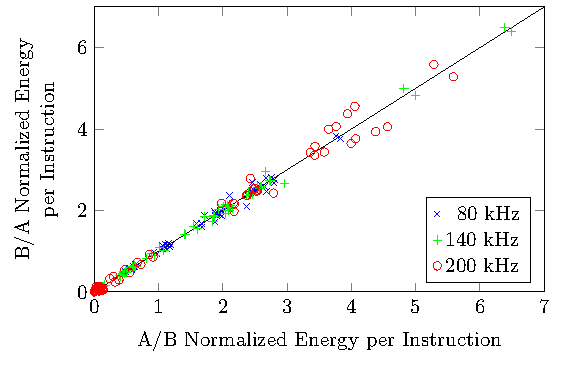
\includegraphics[width=5in]{../TEMC_SAVAT/figures/ab_vs_ba.pdf}
	\caption{ The effect of instruction ordering on observed SAVAT.\label{fig:Order}}
\end{figure}

\subsection{Impact of the Alternation Frequency}\label{sec:freq}

The power spectrum measured close to a desktop or laptop computer consists of numerous peaks protruding above ``rolling hills'' of noise. In addition to intentional radio signals (such as Wifi and Bluetooth), each system has numerous other emanations sources. Switching power supplies create broad noise peaks, clocks create narrow peaks at their operating frequency, and long cables radiate noise across a broad range of frequencies. In addition, moving an EM probe closer to the test system ($<$ 1 meter) reveals that the random switching activities in the processor and other system components create a broadband noise floor (typically higher than the spectrum analyzer noise floor) that varies as a function of frequency.

SAVAT integrates spectral power density over a frequency band around the alternation frequency (5 kHz bandwidth in our experiments), so measuring the same SAVAT value at different alternation frequencies will unavoidably integrate different noise sources along with the intended signal, resulting in different SAVAT values. The emanations created by our benchmarks at the alternation frequency are likely caused by currents flowing through the system's power distribution network (PDN) and are therefore a function of the path this current takes through the PDN. The PDN can be modelled as a network of shunt capacitances and series inductances, and so the current's path is expected to be frequency dependent. A longer current path might enclose a loop with a larger area, creating stronger emanations~\cite{Ott09}. To account for this frequency dependent ``gain'' we normalize by the average SAVAT value at a given frequency when comparing SAVAT across frequencies. For neighboring frequencies (e.g. 80kHz vs 90kHz or 190kHz vs 200kHz), the change in gain is small as shown in Figure~\ref{fig:fdepend} for the DELL Optiplex 7010 desktop with the 20 cm loop antenna. %is this DELL?

\begin{figure}[htb]
	\centering
	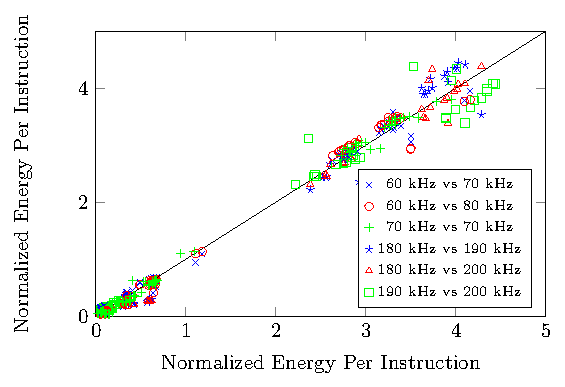
\includegraphics[width=5in]{../TEMC_SAVAT/fdepend.pdf}
	\caption{Comparison of SAVAT at different frequencies for the DELL Optiplex 7010 desktop.}
  \label{fig:fdepend}  
\end{figure}

\begin{figure}[htb]
	\centering
	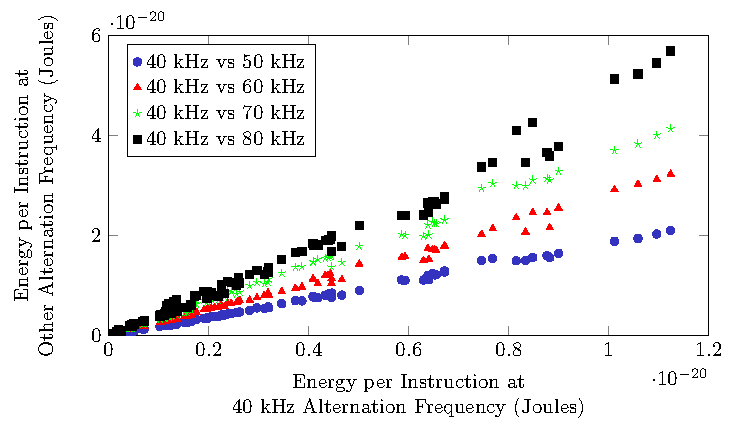
\includegraphics[width=5in]{../emc_comparison_4/freq_depend.pdf}
	\caption{Comparison of SAVATs at different frequencies for NIOS on the DE1 FPGA board. }
  \label{fig:fdepend_nios}
\end{figure}

\begin{figure}[hbt]
	\centering
	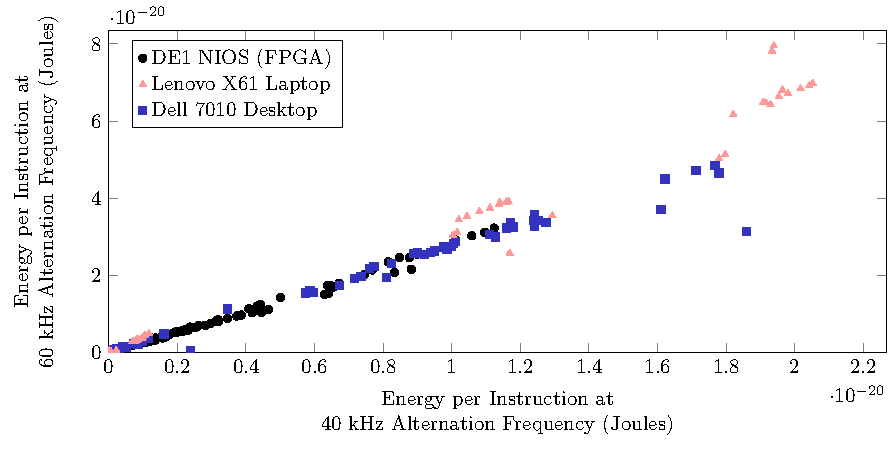
\includegraphics[width=\textwidth]{../emc_comparison_4/freq_depend_compare.pdf}
	\caption{Comparison of SAVATs at 40 kHz and 60 kHz for the NIOS DE1 FPGA, the Lenovo X61 laptop, and the DELL Optiplex 7010 desktop.}   \label{fig:fdepend_compare}
\end{figure}


Figure~\ref{fig:fdepend_nios} shows how SAVAT changes as a function of the alternation frequency on NIOS measured with the 4cm coil probe.% this figure is technically not showing the effect of gain
Each instruction pair is plotted along the x-axis at its SAVAT value measured at 40 kHz, and is plotted along the y-axis at its SAVAT value measured at another frequency. The SAVAT values at 40 kHz appear to be linearly related to the SAVAT values at each other frequency, suggesting that SAVAT values at one frequency can be used to predict SAVAT values at any other frequency in this range. Therefore within this frequency range the DE1 NIOS SAVAT is largely independent of frequency and can be measured at whichever frequency is most convenient. Figure~\ref{fig:fdepend_compare} shows the FPGA SAVAT values at 40 kHz vs 60 kHz, along with the laptop and desktop SAVAT values of comparable magnitude at the same frequencies. All three systems follow a similar trend, suggesting that the SAVAT values on all three systems may have a similar dependence on the measurement frequency.


\begin{comment}
\subsection{Modeling SAVAT Power as a Function of Distance}\label{sec:distance}

To model the sources of these EM emanations and to estimate how far away EM emanations can be received, we need to know how quickly SAVAT decays with distance. Since we are measuring near-field signals using a magnetic loop probe, we expect that the magnetic field will decay as $1/{r^3}$ and that the emanations source can be modelled as a magnetic dipole. However, our measurements did not match this model. Hence, we modelled the side-channel field as a field created by an electric monopole (Hertzian dipole) and a magnetic dipole, where we can receive only magnetic components of the EM field. Hence, the received power can be modelled as
\begin{equation}
	P_r  = {P_t}'\left(\frac{1}{(kr^2)^2}+\frac{1}{(kr^3)^2}\right)
\end{equation}
where \begin{math} k={2\pi}/{\lambda} \end{math} is the wavenumber, \begin{math} {P_t}' \end{math} is a fixed constant to align each theoretical curve to the corresponding power measurement at $0.25$ meters, and $r$ is the distance between the antenna and the system. Figure~\ref{fig:distance} compares theoretical and measured SAVAT for several representative instructions measured at $215~{\rm kHz}$. We observe that the received power of on-chip pairs of instructions (e.g. LDL2/DIV and LDL2/LDL1) decays at the same rate as the received power on-chip/off-chip instruction pairs (e.g. LDL2/STM). Similar agreement between theoretical and measured SAVAT was found at $70~{\rm kHz}$ and $150~{\rm kHz}$.
% using a different r to account for different on-chip and off-chip distance(?)
% mention that this was Core 2 Duo Laptop?
% explain that chose 215 kHz since it had largest magnitude (longest distance)?
% since measurement is normalized at 25cm, the effect of k is cancelled out

\begin{figure}[htb]
	\centering
	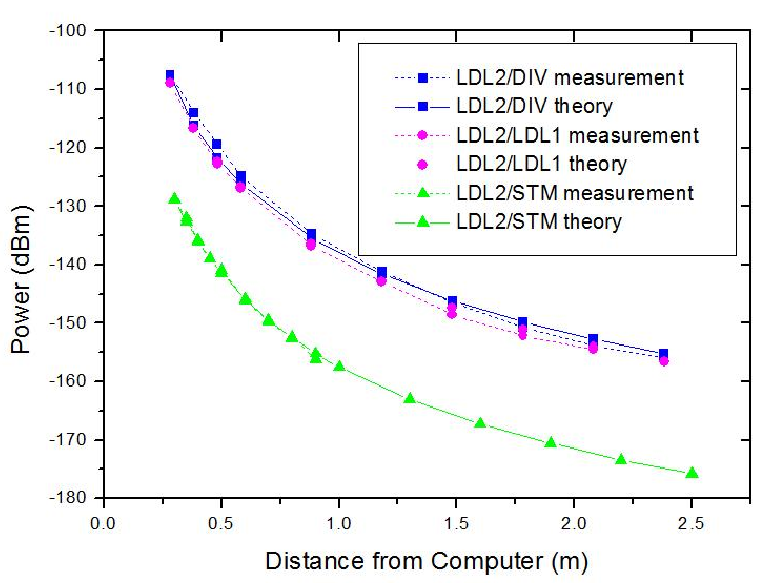
\includegraphics[width=5in]{../TEMC_SAVAT/distance1.pdf}
	\caption{SAVAT as a function of measurement distance.}
\label{fig:distance}    
\end{figure}
\end{comment}
